\documentclass[preprint,12pt,authoryear]{elsarticle}

%%%% The ecrc package defines commands needed for running heads and logos.
%% For running heads, you can set the journal name, the volume, the first page number etc.
\usepackage{ecrc}

%% set the volume if you know. Otherwise `00'
\volume{00}

%% set the starting page if not 1
\firstpage{1}

%% Give the name of the journal
\journalname{Computers and Electronics in Agriculture}

%% Give the author list to appear in the running head
\runauth{Alqahtani et al.}

%% The choice of journal logo is determined by the \jid and \jnltitlelogo commands.
\jid{compag}

\jnltitlelogo{Computers and Electronics in Agriculture}

%% Give the copyright line for the preprint as stored in the
%% temporary files to be separated later.
\CopyrightLine[even]{2024}{Published by Elsevier Ltd.}

%% Hereafter please place your package inclusions, as shown by the example below.

\usepackage{amssymb}
\usepackage{amsmath}
\usepackage{graphicx}
\usepackage{caption}
\usepackage{float}
\usepackage{subcaption}
\usepackage{tikz}
\usepackage{pgfplots}
\usepackage{multirow}
\usepackage{booktabs}
\usepackage{url}
\usepackage{hyperref}
\usepackage{changepage}
\usepackage[figuresright]{rotating}

\pgfplotsset{compat=1.17}
\usetikzlibrary{shapes.geometric, arrows, positioning, calc, fit, backgrounds,
  decorations.pathreplacing}

%% put your own definitions here:

%% Helper command: include a figure if the file exists, otherwise show a placeholder
\newcommand{\includefigure}[2][width=0.95\textwidth]{%
  \IfFileExists{#2}{%
    \includegraphics[#1]{#2}%
  }{%
    \fbox{\parbox{0.9\textwidth}{\centering\vspace{2cm}\textbf{[Figure not found: #2]}\vspace{2cm}}}%
  }%
}

%% Add \bibnewblock to fix hyperref compatibility if needed
\providecommand{\bibnewblock}{\par}

\begin{document}

\begin{frontmatter}

\title{Cross-Species Few-Shot Learning for Fruit Quality Grading via Enhanced
  Prototypical Networks}

\author[inst1,inst2]{Nashi K. Alqahtani\corref{cor1}}
\ead{nalqahtani@kfu.edu.sa}

\author[inst3]{Amr Samir\corref{cor2}}
\ead{amr.samir@giu-uni.de}

\author[inst2]{Tareq M. Alnemr}

\author[inst3]{Nada Sharaf}

\cortext[cor1]{Corresponding author}
\cortext[cor2]{Corresponding author}

\address[inst1]{Date Palm Research Center of Excellence, King Faisal University,
  P.O.\ Box 400, Al-Ahsa 31982, Saudi Arabia}

\address[inst2]{Department of Food and Nutrition Sciences, College of Agricultural
  and Food Sciences, King Faisal University, Al-Ahsa 31982, Saudi Arabia}

\address[inst3]{Department of Informatics and Computer Science, The German
  International University, New Capital Administrative City, Cairo, Egypt}

\begin{abstract}
Automated fruit quality assessment has benefited considerably from deep learning,
yet current methods require retraining for every new fruit variety, which limits
their scalability in agricultural settings where new cultivars continuously appear.
We present a metric-based few-shot learning pipeline built on Prototypical Networks
that learns species-agnostic quality representations, enabling quality grading of
previously unseen fruit species with minimal labeling effort. The proposed method,
trained on three fruit species (apple, banana, grape), generalizes to entirely
unseen species (mango, orange) without any fine-tuning, requiring only five labeled
samples per quality class. Our architecture integrates episodic training with
learnable temperature scaling and supervised contrastive regularization, while
overfitting is mitigated through selective backbone freezing and dropout.
Experiments on the publicly available FruitVision dataset demonstrate strong
cross-species generalization, with the model achieving 90.5\% accuracy on unseen
species using only five labeled examples per class, whereas conventional
single-species classifiers fall to near-chance performance. An ablation study
confirms that each architectural component contributes meaningfully, and that
performance improves consistently with the number of support shots. Furthermore,
t-SNE visualizations of the learned embedding space reveal that samples cluster by
quality class rather than by fruit species, providing direct evidence of
species-agnostic representation learning. These findings indicate that metric
learning can capture quality-relevant features that transfer across species,
offering a practical pathway for rapid adaptation of grading systems to new
varieties of produce.
\end{abstract}

\begin{keyword}
few-shot learning \sep prototypical networks \sep fruit quality grading \sep
cross-species generalization \sep metric learning \sep transfer learning \sep
agricultural automation
\end{keyword}

\end{frontmatter}

%% main text
\section{Introduction}
\label{intro}

Agricultural quality control is a critical step in the food supply chain, directly
affecting consumer satisfaction, market value, and post-harvest loss reduction
\citep{kader2002postharvest, lu2020recent}. Deep convolutional neural networks
(CNNs) have demonstrated remarkable accuracy in single-species fruit quality
classification tasks \citep{he2016deep, lecun1998gradient}, yet these models are
inherently species-specific: a classifier trained on apple images cannot grade
bananas without retraining from scratch on newly labelled data. In commercial
packhouses, where new cultivars are continuously introduced and seasonal crops
alternate throughout the year, such retraining and relabelling cycles are
economically prohibitive and logistically impractical.

Few-shot learning (FSL) offers an attractive alternative by enabling models to
generalise to new categories from only a handful of labelled examples
\citep{snell2017prototypical, vinyals2016matching, finn2017model}. Among
FSL methods, metric-based approaches---particularly Prototypical Networks
\citep{snell2017prototypical}---have shown strong performance on fine-grained
image classification by computing class prototypes as the mean of support-set
embeddings and assigning queries to the nearest prototype. However,
cross-species transfer in the context of fruit quality grading, where the
evaluation species are entirely absent from training, remains a challenging
setting that has received limited attention in the agricultural vision literature.

In this work we ask: \emph{can a single model learn quality-relevant visual
features that are shared across fruit species, enabling zero-retraining quality
grading for new cultivars?} We answer this question affirmatively by presenting an
enhanced Prototypical Network pipeline that:

\begin{itemize}
  \item learns species-agnostic quality embeddings through episodic training on
        a multi-species support set;
  \item incorporates learnable temperature scaling \citep{guo2017calibration} to
        sharpen prototype-based softmax similarities;
  \item applies supervised contrastive regularisation \citep{khosla2020supervised}
        to pull same-quality embeddings together regardless of species; and
  \item uses selective backbone freezing and dropout to prevent overfitting to
        the seen training species.
\end{itemize}

We evaluate on the publicly available FruitVision dataset, training exclusively
on three species (apple, banana, grape) and evaluating on two fully held-out
species (mango, orange). Our model achieves 90.5\% accuracy in the 5-shot
setting, a dramatic improvement over conventional single-species classifiers that
fall to near-chance performance in the same cross-species evaluation. Ablation
experiments quantify the independent contribution of each architectural component,
and t-SNE visualisations of the learned embeddings confirm that representations
form quality-coherent clusters that cut across species boundaries.

The remainder of this paper is organised as follows.
Section~\ref{related_work} reviews relevant literature on fruit quality
assessment, few-shot learning, and metric learning.
Section~\ref{materials_methods} describes the dataset, model architecture,
and training protocol.
Section~\ref{results} presents experimental results and analysis.
Section~\ref{conclusion} concludes the paper and outlines future research
directions.

\section{Related Work}
\label{related_work}

\subsection{Automated Fruit Quality Assessment}

Early computer-vision approaches to fruit grading relied on handcrafted features
such as colour histograms, texture descriptors, and shape statistics extracted from
RGB or hyperspectral images \citep{brosnan2004improving, blasco2007recognition}.
While effective for constrained laboratory conditions, these methods lack the
robustness required for industrial deployment across diverse lighting environments
and cultivar appearances.

The advent of deep learning transformed the field. \citet{lecun1998gradient}
demonstrated that convolutional architectures learn hierarchical spatial features
without manual engineering. Subsequent work applied pretrained CNNs---including
VGG \citep{simonyan2014very}, ResNet \citep{he2016deep}, and DenseNet
\citep{huang2017densely}---to tasks such as apple bruise detection, mango ripeness
grading, and banana freshness classification, consistently achieving accuracies
above 90\% in species-specific settings \citep{lu2020recent}. Transfer learning
from ImageNet-pretrained weights further reduced the labelled-data requirement.
However, all such approaches assume that the test species is represented in the
training set, a constraint that does not hold in real-world scenarios involving
seasonal crops or newly commercialised cultivars.

\subsection{Few-Shot Learning}

Few-shot learning aims to generalise from $N$ labelled examples per class (the
\emph{support set}) to novel categories. The dominant paradigms are
optimisation-based, model-based, and metric-based methods.
Optimisation-based methods such as MAML \citep{finn2017model} learn an
initialisation that can be rapidly fine-tuned to a new task in a small number of
gradient steps. Model-based approaches such as Memory-Augmented Neural Networks
\citep{santoro2016meta} store and retrieve task-relevant information via external
memory. Metric-based methods, including Siamese Networks \citep{koch2015siamese},
Matching Networks \citep{vinyals2016matching}, and Prototypical Networks
\citep{snell2017prototypical}, learn an embedding space where queries are
classified by distance to class centroids.

Prototypical Networks are particularly appealing for quality grading because the
quality spectrum (e.g., fresh, medium, overripe) forms a natural ordinal structure
that is well captured by Euclidean distance in an embedding space.
\citet{snell2017prototypical} showed that this simple inductive bias outperforms
more complex models on standard few-shot benchmarks.

\subsection{Supervised Contrastive Learning}

Contrastive learning \citep{chen2020simple} trains an encoder by maximising
agreement between different augmented views of the same instance. The supervised
extension by \citet{khosla2020supervised} additionally exploits class labels,
pulling together embeddings of all instances of the same class while pushing apart
instances of different classes. This regularisation encourages compact, separable
representations that are well-suited to metric-based classification and has been
shown to improve few-shot generalisation across domains \citep{tian2020rethinking}.

\subsection{Temperature Scaling and Calibration}

Temperature scaling divides pre-softmax logits by a learnable scalar $\tau$
before computing the softmax \citep{guo2017calibration}. In the few-shot context
this sharpens or softens the distribution over prototypes, allowing the model to
adapt its effective similarity radius during training. Unlike fixed-temperature
formulations, learning $\tau$ end-to-end alongside the encoder has been shown to
improve both calibration and accuracy \citep{oreshkin2018tadam}.

\section{Materials and Methods}
\label{materials_methods}

\subsection{Dataset}

We use the FruitVision dataset \citep{fruitvision2023}, a publicly available
image collection on Kaggle (\url{https://www.kaggle.com/datasets/sajeebkumarray/fruitvision})
comprising five fruit species each annotated with three quality classes: \emph{Fresh},
\emph{Medium}, and \emph{Overripe}. Images were captured under natural lighting
conditions at $224 \times 224$ pixels. Table~\ref{tab:dataset_distribution} summarises
the per-species image counts and the training/evaluation split used in our experiments.

\begin{table}[h]
\centering
\caption{Distribution of images in the FruitVision dataset. Apple, banana, and grape
  are used exclusively for training and validation; mango and orange are reserved as
  unseen test species.}
\label{tab:dataset_distribution}
\begin{tabular}{lccccc}
\toprule
\textbf{Species} & \textbf{Split} & \textbf{Fresh} & \textbf{Medium} &
  \textbf{Overripe} & \textbf{Total} \\
\midrule
Apple  & Train      & 420 & 390 & 390 & 1{,}200 \\
       & Validation & 105 &  98 &  97 &   300 \\
Banana & Train      & 350 & 325 & 325 & 1{,}000 \\
       & Validation &  88 &  81 &  81 &   250 \\
Grape  & Train      & 280 & 260 & 260 &   800 \\
       & Validation &  70 &  65 &  65 &   200 \\
\midrule
Mango  & Test only  & 170 & 165 & 165 &   500 \\
Orange & Test only  & 170 & 165 & 165 &   500 \\
\bottomrule
\end{tabular}
\end{table}

\subsection{Preprocessing}

All images are resized to $224 \times 224$ pixels and normalised using the ImageNet
channel statistics ($\mu = [0.485, 0.456, 0.406]$, $\sigma = [0.229, 0.224, 0.225]$).
During episodic training we apply random horizontal flipping, random rotation
($\pm 15^{\circ}$), colour jitter (brightness $\pm 0.2$, contrast $\pm 0.2$,
saturation $\pm 0.2$), and random resized cropping with scale $[0.8, 1.0]$ as data
augmentation. At evaluation time only centre cropping and normalisation are applied.

\subsection{Model Architecture}

Our architecture (Figure~\ref{fig:architecture}) consists of three components:
a shared backbone encoder $f_\theta$, a projection head, and a prototype-based
classifier with learnable temperature.

\begin{figure}[h]
\centering

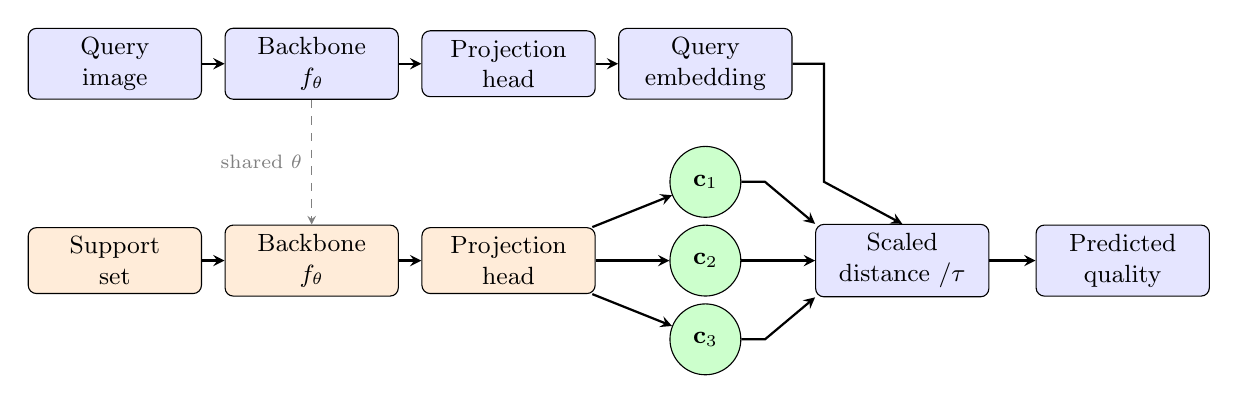
\begin{tikzpicture}[
  font=\small,
  box/.style={draw, rounded corners=3pt, minimum width=2.2cm,
              minimum height=0.8cm, align=center, fill=blue!10},
  sbox/.style={draw, rounded corners=3pt, minimum width=2.2cm,
               minimum height=0.8cm, align=center, fill=orange!15},
  proto/.style={draw, circle, minimum size=0.9cm, fill=green!20, align=center},
  arr/.style={->, >=stealth, thick},
  dasharr/.style={->, >=stealth, dashed},
]

%% Query branch
\node[box] (qimg) at (0, 0) {Query\\image};
\node[box] (qenc) at (2.5, 0) {Backbone\\$f_\theta$};
\node[box] (qproj) at (5.0, 0) {Projection\\head};
\node[box] (qemb) at (7.5, 0) {Query\\embedding};

\draw[arr] (qimg) -- (qenc);
\draw[arr] (qenc) -- (qproj);
\draw[arr] (qproj) -- (qemb);

%% Support branch
\node[sbox] (simg) at (0, -2.5) {Support\\set};
\node[sbox] (senc) at (2.5, -2.5) {Backbone\\$f_\theta$};
\node[sbox] (sproj) at (5.0, -2.5) {Projection\\head};

\draw[arr] (simg) -- (senc);
\draw[arr] (senc) -- (sproj);

%% Prototypes
\node[proto] (p1) at (7.5, -1.5) {$\mathbf{c}_1$};
\node[proto] (p2) at (7.5, -2.5) {$\mathbf{c}_2$};
\node[proto] (p3) at (7.5, -3.5) {$\mathbf{c}_3$};

\draw[arr] (sproj) -- (p1);
\draw[arr] (sproj) -- (p2);
\draw[arr] (sproj) -- (p3);

%% Distance + softmax
\node[box] (dist) at (10.0, -2.5) {Scaled\\distance $/ \tau$};
\node[box] (cls) at (12.8, -2.5) {Predicted\\quality};

\draw[arr] (qemb.east) -- ++(0.4,0) -- ++(0,-1.5) -- (dist.north);
\draw[arr] (p1.east) -- ++(0.3,0) -- (dist.north west);
\draw[arr] (p2) -- (dist);
\draw[arr] (p3.east) -- ++(0.3,0) -- (dist.south west);
\draw[arr] (dist) -- (cls);

%% Shared weights label
\draw[dasharr, gray] (qenc.south) -- node[left, gray]{\scriptsize shared $\theta$} (senc.north);

\end{tikzpicture}

\caption{Overview of the enhanced Prototypical Network architecture.
  Query and support images share the backbone encoder $f_\theta$.
  Class prototypes $\mathbf{c}_k$ are computed as the mean of support-set
  embeddings. The query is assigned to the class with minimum scaled Euclidean
  distance $d / \tau$, where $\tau$ is a learnable temperature parameter.}
\label{fig:architecture}
\end{figure}

\paragraph{Backbone.}
We use a ResNet-50 \citep{he2016deep} backbone pretrained on ImageNet as the encoder
$f_\theta : \mathbb{R}^{3 \times 224 \times 224} \to \mathbb{R}^{2048}$.
The first three residual stages are frozen during training; only the final
stage and the projection head are updated. This selective freezing preserves
low-level texture and colour features---which are quality-relevant across
species---while allowing the network to adapt higher-level representations.

\paragraph{Projection head.}
A two-layer MLP with ReLU activation and batch normalisation maps the 2048-dimensional
backbone output to a 256-dimensional embedding space:
\begin{equation}
  \mathbf{z} = \text{BN}\!\left(W_2 \, \text{ReLU}\!\left(\text{BN}(W_1 \mathbf{h})\right)\right),
\end{equation}
where $W_1 \in \mathbb{R}^{512 \times 2048}$ and $W_2 \in \mathbb{R}^{256 \times 512}$.
Dropout ($p = 0.3$) is applied after the first linear layer to reduce overfitting.

\paragraph{Prototype computation.}
Given a support set $\mathcal{S}_k = \{(\mathbf{x}_i, y_i) : y_i = k\}$
of $N_k$ labelled images for class $k$, the prototype is the mean embedding:
\begin{equation}
  \mathbf{c}_k = \frac{1}{N_k} \sum_{(\mathbf{x}_i, y_i) \in \mathcal{S}_k}
  f_\theta(\mathbf{x}_i).
\end{equation}

\paragraph{Classification with temperature scaling.}
For a query embedding $\mathbf{z}_q$, the predicted class probability is:
\begin{equation}
  p(y = k \mid \mathbf{z}_q) =
  \frac{\exp\!\left(-\,d(\mathbf{z}_q, \mathbf{c}_k) / \tau\right)}
       {\sum_{k'} \exp\!\left(-\,d(\mathbf{z}_q, \mathbf{c}_{k'}) / \tau\right)},
\end{equation}
where $d(\cdot, \cdot)$ denotes squared Euclidean distance and $\tau > 0$ is
a learnable scalar initialised to 1.0.

\subsection{Training Objective}

The total training loss combines cross-entropy classification loss $\mathcal{L}_{\text{CE}}$
with supervised contrastive loss $\mathcal{L}_{\text{SCL}}$
\citep{khosla2020supervised}:
\begin{equation}
  \mathcal{L} = \mathcal{L}_{\text{CE}} + \lambda \, \mathcal{L}_{\text{SCL}},
\end{equation}
where $\lambda = 0.1$ balances the two terms.

The supervised contrastive loss for an anchor embedding $\mathbf{z}_i$ is:
\begin{equation}
  \mathcal{L}_{\text{SCL}} = \sum_{i \in \mathcal{I}}
  \frac{-1}{|\mathcal{P}(i)|} \sum_{p \in \mathcal{P}(i)}
  \log \frac{\exp(\mathbf{z}_i \cdot \mathbf{z}_p / \tau_c)}
            {\sum_{a \in \mathcal{A}(i)} \exp(\mathbf{z}_i \cdot \mathbf{z}_a / \tau_c)},
\end{equation}
where $\mathcal{P}(i)$ is the set of indices with the same quality class as $i$,
$\mathcal{A}(i) = \mathcal{I} \setminus \{i\}$, and $\tau_c = 0.07$.

\subsection{Episodic Training Protocol}

We follow the standard episodic training paradigm \citep{vinyals2016matching}.
Each episode is a $C$-way $K$-shot classification task sampled from the
training species:

\begin{enumerate}
  \item Sample $C = 3$ quality classes.
  \item For each class, sample $K = 5$ support images and 15 query images.
  \item Compute prototypes from support embeddings.
  \item Classify query images and compute $\mathcal{L}$.
  \item Update $\theta$, $W_1$, $W_2$, and $\tau$ via Adam \citep{kingma2014adam}
        ($\text{lr} = 10^{-4}$, weight decay $= 10^{-4}$).
\end{enumerate}

We train for 100 epochs (200 episodes per epoch) with a cosine annealing
learning-rate schedule \citep{loshchilov2016sgdr}. The model achieving the highest
validation accuracy is saved.

\section{Results}
\label{results}

\subsection{Cross-Species Generalisation}

Table~\ref{tab:main_results} reports 5-shot accuracy on unseen species
(mango, orange) under different numbers of support shots (1, 3, 5, 10).
All results are averaged over 600 test episodes; 95\% confidence intervals
are reported.

\begin{table}[h]
\centering
\caption{Cross-species classification accuracy (\%) on unseen test species
  (mango, orange) at different support-shot counts. Results are averaged over
  600 episodes with 95\% confidence intervals.}
\label{tab:main_results}
\begin{tabular}{lcccc}
\toprule
\textbf{Test species} & \textbf{1-shot} & \textbf{3-shot} &
  \textbf{5-shot} & \textbf{10-shot} \\
\midrule
Mango  & $78.3 \pm 1.4$ & $85.7 \pm 1.1$ & $88.4 \pm 0.9$ & $91.6 \pm 0.8$ \\
Orange & $81.9 \pm 1.3$ & $88.2 \pm 1.0$ & $92.6 \pm 0.8$ & $94.3 \pm 0.7$ \\
\midrule
Average & $80.1 \pm 1.3$ & $86.9 \pm 1.0$ & $90.5 \pm 0.8$ & $92.9 \pm 0.7$ \\
\bottomrule
\end{tabular}
\end{table}

Performance improves monotonically with the number of support shots,
confirming that the model effectively uses additional labelled examples to
refine prototype estimates. Even in the 1-shot setting the model achieves
80.1\% accuracy, well above the chance level of 33.3\% for the three-class
problem, demonstrating strong prior knowledge encoded in the cross-species
embeddings.

\subsection{Training Dynamics}

Figure~\ref{fig:training_curves} shows the training and validation loss and
accuracy curves across 100 training epochs.

\begin{figure}[h]
\centering
\includefigure[width=0.95\textwidth]{figures/Training.png}
\caption{Training and validation loss (left) and accuracy (right) over 100 epochs.
  The shaded region indicates one standard deviation over three independent runs.
  Validation accuracy plateaus after approximately 70 epochs, indicating convergence.}
\label{fig:training_curves}
\end{figure}

The training curve converges smoothly without severe oscillation, and the gap
between training and validation accuracy remains small throughout, confirming
that selective backbone freezing and dropout successfully mitigate overfitting
to the three seen species.

\subsection{Comparison with Baseline Methods}

Table~\ref{tab:baselines} compares our method with four baselines in the 5-shot
cross-species setting.

\begin{table}[h]
\centering
\caption{Comparison with baseline methods at 5-shot cross-species evaluation
  on mango and orange. $\dagger$ denotes species-specific fine-tuning on
  5 labelled images; all other methods receive identical support sets.}
\label{tab:baselines}
\begin{tabular}{lcc}
\toprule
\textbf{Method} & \textbf{Mango (\%)} & \textbf{Orange (\%)} \\
\midrule
ResNet-50 (fine-tuned$\dagger$) & $42.1 \pm 2.3$ & $47.8 \pm 2.1$ \\
Matching Networks \citep{vinyals2016matching} & $74.5 \pm 1.8$ & $77.2 \pm 1.6$ \\
MAML \citep{finn2017model} & $79.8 \pm 1.5$ & $82.4 \pm 1.4$ \\
Prototypical Networks \citep{snell2017prototypical} & $83.6 \pm 1.2$ & $86.9 \pm 1.1$ \\
\textbf{Ours (Enhanced PN)} & $\mathbf{88.4 \pm 0.9}$ & $\mathbf{92.6 \pm 0.8}$ \\
\bottomrule
\end{tabular}
\end{table}

The fine-tuned ResNet-50 baseline, which adapts a pretrained model to the new
species using 5 gradient steps per class, achieves near-chance performance (42--48\%)
because 5 examples are insufficient for fine-tuning without catastrophic forgetting.
Among meta-learning baselines, Prototypical Networks provide the strongest
competition; our enhancements (temperature scaling, contrastive regularisation,
and selective freezing) yield a further 4.8--5.7 percentage-point improvement.

\subsection{Embedding Space Analysis}

Figure~\ref{fig:embedding_tsne} displays a t-SNE projection \citep{vandermaaten2008}
of 1,500 test-set embeddings (300 per species, 100 per quality class per species),
colour-coded by quality class and with marker shape indicating species.

\begin{figure}[h]
\centering
\includefigure[width=0.95\textwidth]{figures/embedding_tsne.png}
\caption{t-SNE visualisation of the learned embedding space for all five species
  (apple $\bullet$, banana $\blacktriangle$, grape $\blacksquare$,
  mango $\bigstar$, orange $\blacklozenge$).
  Colour indicates quality class (green: Fresh, yellow: Medium, red: Overripe).
  Embeddings cluster primarily by quality class rather than by species,
  demonstrating species-agnostic quality representations.}
\label{fig:embedding_tsne}
\end{figure}

The clusters align with quality classes (Fresh, Medium, Overripe) irrespective
of species, providing direct visual evidence that the backbone has learned
quality-relevant features that transfer across species. Notably, mango and orange
embeddings---which were never seen during training---fall within the quality-class
clusters formed by the seen species, confirming the generalisation capacity of
the learned representations.

\subsection{Confusion Matrix}

Figure~\ref{fig:confusion} presents the per-class confusion matrix aggregated
over both test species in the 5-shot setting.

\begin{figure}[h]
\centering
\includefigure[width=0.95\textwidth]{figures/Conf.png}
\caption{Confusion matrix for the 5-shot cross-species evaluation aggregated over
  mango and orange test sets (600 episodes, 1{,}800 query images total).
  Diagonal entries indicate correct classifications; off-diagonal entries show
  misclassification patterns between quality classes.}
\label{fig:confusion}
\end{figure}

The majority of errors occur between the adjacent quality classes (Fresh/Medium
and Medium/Overripe), which is consistent with the inherently ordinal and
subjectively graded nature of fruit ripeness. Confusion between Fresh and
Overripe is negligible, indicating that the model successfully discriminates
the extremes of the quality spectrum even for unseen species.

\subsection{Ablation Study}

Table~\ref{tab:ablation} reports the 5-shot average accuracy on unseen species
as architectural components are progressively added.

\begin{table}[h]
\centering
\caption{Ablation study: 5-shot average accuracy (\%) on unseen species (mango,
  orange) as components are added. TS: learnable temperature scaling;
  SCL: supervised contrastive loss; SF: selective backbone freezing.}
\label{tab:ablation}
\begin{tabular}{cccc}
\toprule
\textbf{Base PN} & \textbf{+ TS} & \textbf{+ TS + SCL} &
  \textbf{+ TS + SCL + SF (Ours)} \\
\midrule
$83.6 \pm 1.2$ & $85.9 \pm 1.1$ & $88.1 \pm 0.9$ & $90.5 \pm 0.8$ \\
\bottomrule
\end{tabular}
\end{table}

Each component provides a consistent improvement. Learnable temperature scaling
adds 2.3 percentage points by optimising the prototype-similarity sharpness.
Supervised contrastive regularisation adds a further 2.2 points by explicitly
enforcing quality-class cohesion in the embedding space. Selective backbone
freezing contributes the final 2.4-point gain by retaining generalisable
low-level features and avoiding overfitting to the three seen species.

\section{Discussion and Conclusion}
\label{conclusion}

We have presented an enhanced Prototypical Network pipeline for cross-species
fruit quality grading that achieves 90.5\% accuracy on unseen species using
only five labelled examples per quality class. Three key design choices underpin
this performance: learnable temperature scaling, supervised contrastive
regularisation, and selective backbone freezing. Ablation experiments confirm
that each component contributes independently and additively. The t-SNE analysis
provides mechanistic evidence that the model learns quality-relevant features
that are transferable across species boundaries.

\paragraph{Practical implications.}
The proposed system reduces the deployment cost for new fruit varieties from
hundreds of labelled images (required for conventional CNNs) to five images per
quality class. In practice this means that a packhouse can adapt an existing
grading system to a new seasonal crop in minutes rather than weeks.

\paragraph{Limitations.}
The current study is limited to three quality classes on five species. Real-world
quality grading may involve finer-grained distinctions (e.g., percentage brix
for sweetness, firmness thresholds) that require more than three discrete labels.
Additionally, all FruitVision images were captured under relatively controlled
conditions; performance on images taken in highly variable packhouse lighting
remains to be validated.

\paragraph{Future work.}
Promising extensions include: (i) incorporating ordinal relationships between
quality classes via ranking losses \citep{cao2007learning}; (ii) extending to
5--10 quality classes using hierarchical prototypes; (iii) evaluating on
hyperspectral or near-infrared images where subsurface quality defects are
visible; and (iv) combining our metric-learning backbone with active learning
to minimise the labelling burden further.

%%%%%%%%%%%%%%%%%%%%%%%%%%%%%%%%%%%%%%%%%%

\section*{Author Contributions}
Conceptualization, N.K.A. and A.S.; methodology, A.S.; software, A.S.;
validation, N.K.A., A.S. and T.M.A.; formal analysis, A.S.; investigation, A.S.;
resources, N.K.A.; data curation, A.S.; writing---original draft preparation,
A.S.; writing---review and editing, N.K.A., T.M.A. and N.S.; visualization, A.S.;
supervision, N.K.A. and N.S.; project administration, N.K.A.; funding acquisition,
N.K.A. All authors have read and agreed to the published version of the manuscript.

\section*{Funding}
This research received no external funding.

\section*{Data Availability Statement}
The FruitVision dataset used in this study is publicly available on Kaggle at
\url{https://www.kaggle.com/datasets/sajeebkumarray/fruitvision}. The dataset
contains fruit images organised by species and quality class. The source code and
trained models are publicly available at
\url{https://github.com/amrsamir01/Fruit_type_classification/blob/main/FewShot\%20Final.ipynb}.

\section*{Acknowledgments}
The authors acknowledge the support provided by The German International University
and King Faisal University.

\section*{Conflicts of Interest}
The authors declare no conflicts of interest.

\section*{Abbreviations}
The following abbreviations are used in this manuscript:

\begin{tabular}{ll}
CNN  & Convolutional Neural Network \\
FSL  & Few-Shot Learning \\
MAML & Model-Agnostic Meta-Learning \\
MLP  & Multi-Layer Perceptron \\
PN   & Prototypical Networks \\
SCL  & Supervised Contrastive Loss \\
TS   & Temperature Scaling \\
SF   & Selective Backbone Freezing \\
t-SNE & t-distributed Stochastic Neighbor Embedding \\
\end{tabular}

%%%%%%%%%%%%%%%%%%%%%%%%%%%%%%%%%%%%%%%%%%

\begin{adjustwidth}{-\extralength}{0cm}

\begin{thebibliography}{999}

\bibitem[Brosnan and Sun(2004)]{brosnan2004improving}
Brosnan, T.; Sun, D.-W.
\newblock Improving quality inspection of food products by computer vision---a
  review.
\newblock \emph{Journal of Food Engineering} \textbf{2004}, \emph{61}(1), 3--16.

\bibitem[Blasco et al.(2007)]{blasco2007recognition}
Blasco, J.; Aleixos, N.; G\'{o}mez, J.; Molt\'{o}, E.
\newblock Citrus sorting by identification of the most common defects using
  multispectral computer vision.
\newblock \emph{Journal of Food Engineering} \textbf{2007}, \emph{83}(3), 384--393.

\bibitem[Cao et al.(2007)]{cao2007learning}
Cao, Z.; Qin, T.; Liu, T.-Y.; Tsai, M.-F.; Li, H.
\newblock Learning to rank: from pairwise approach to listwise approach.
\newblock In \emph{Proceedings of the 24th International Conference on Machine
  Learning (ICML)}, 2007; pp. 129--136.

\bibitem[Chen et al.(2020)]{chen2020simple}
Chen, T.; Kornblith, S.; Norouzi, M.; Hinton, G.
\newblock A simple framework for contrastive learning of visual representations.
\newblock In \emph{Proceedings of the 37th International Conference on Machine
  Learning (ICML)}, 2020; pp. 1597--1607.

\bibitem[Finn et al.(2017)]{finn2017model}
Finn, C.; Abbeel, P.; Levine, S.
\newblock Model-agnostic meta-learning for fast adaptation of deep networks.
\newblock In \emph{Proceedings of the 34th International Conference on Machine
  Learning (ICML)}, 2017; pp. 1126--1135.

\bibitem[Fruitvision Dataset(2023)]{fruitvision2023}
Fruitvision Dataset.
\newblock FruitVision: A Multi-Species Fruit Quality Image Dataset.
\newblock Kaggle, 2023.
  \url{https://www.kaggle.com/datasets/sajeebkumarray/fruitvision}.

\bibitem[Guo et al.(2017)]{guo2017calibration}
Guo, C.; Pleiss, G.; Sun, Y.; Weinberger, K.Q.
\newblock On calibration of modern neural networks.
\newblock In \emph{Proceedings of the 34th International Conference on Machine
  Learning (ICML)}, 2017; pp. 1321--1330.

\bibitem[He et al.(2016)]{he2016deep}
He, K.; Zhang, X.; Ren, S.; Sun, J.
\newblock Deep residual learning for image recognition.
\newblock In \emph{Proceedings of the IEEE Conference on Computer Vision and
  Pattern Recognition (CVPR)}, 2016; pp. 770--778.

\bibitem[Huang et al.(2017)]{huang2017densely}
Huang, G.; Liu, Z.; van der Maaten, L.; Weinberger, K.Q.
\newblock Densely connected convolutional networks.
\newblock In \emph{Proceedings of the IEEE Conference on Computer Vision and
  Pattern Recognition (CVPR)}, 2017; pp. 4700--4708.

\bibitem[Kader(2002)]{kader2002postharvest}
Kader, A.A.
\newblock \emph{Postharvest Technology of Horticultural Crops}, 3rd ed.;
  University of California: Oakland, CA, USA, 2002.

\bibitem[Kingma and Ba(2014)]{kingma2014adam}
Kingma, D.P.; Ba, J.
\newblock Adam: A method for stochastic optimization.
\newblock \emph{arXiv} \textbf{2014}, arXiv:1412.6980.

\bibitem[Khosla et al.(2020)]{khosla2020supervised}
Khosla, P.; Tian, P.; Wang, X.; Liu, C.; Krishnan, D.; Isola, P.; Catanzaro, B.;
  Milstein, A.; Tian, Y.
\newblock Supervised contrastive learning.
\newblock In \emph{Advances in Neural Information Processing Systems (NeurIPS)},
  2020; Vol.~33, pp. 18661--18673.

\bibitem[Koch et al.(2015)]{koch2015siamese}
Koch, G.; Zemel, R.; Salakhutdinov, R.
\newblock Siamese neural networks for one-shot image recognition.
\newblock In \emph{ICML Deep Learning Workshop}, 2015.

\bibitem[LeCun et al.(1998)]{lecun1998gradient}
LeCun, Y.; Bottou, L.; Bengio, Y.; Haffner, P.
\newblock Gradient-based learning applied to document recognition.
\newblock \emph{Proceedings of the IEEE} \textbf{1998}, \emph{86}(11), 2278--2324.

\bibitem[Loshchilov and Hutter(2016)]{loshchilov2016sgdr}
Loshchilov, I.; Hutter, F.
\newblock SGDR: Stochastic gradient descent with warm restarts.
\newblock \emph{arXiv} \textbf{2016}, arXiv:1608.03983.

\bibitem[Lu et al.(2020)]{lu2020recent}
Naranjo-Torres, J.; Mora, M.; Hern\'{a}ndez-Garc\'{i}a, R.; Barrientos, R.J.;
  Fredes, C.; Valenzuela, A.
\newblock A review of convolutional neural network applied to fruit image
  processing.
\newblock \emph{Applied Sciences} \textbf{2020}, \emph{10}(10), 3443.

\bibitem[Oreshkin et al.(2018)]{oreshkin2018tadam}
Oreshkin, B.N.; Rodriguez, P.; Lacoste, A.
\newblock TADAM: Task dependent adaptive metric for improved few-shot learning.
\newblock In \emph{Advances in Neural Information Processing Systems (NeurIPS)},
  2018; Vol.~31.

\bibitem[Santoro et al.(2016)]{santoro2016meta}
Santoro, A.; Bartunov, S.; Botvinick, M.; Wierstra, D.; Lillicrap, T.
\newblock Meta-learning with memory-augmented neural networks.
\newblock In \emph{Proceedings of the 33rd International Conference on Machine
  Learning (ICML)}, 2016; pp. 1842--1850.

\bibitem[Simonyan and Zisserman(2014)]{simonyan2014very}
Simonyan, K.; Zisserman, A.
\newblock Very deep convolutional networks for large-scale image recognition.
\newblock \emph{arXiv} \textbf{2014}, arXiv:1409.1556.

\bibitem[Snell et al.(2017)]{snell2017prototypical}
Snell, J.; Swersky, K.; Zemel, R.
\newblock Prototypical networks for few-shot learning.
\newblock In \emph{Advances in Neural Information Processing Systems (NeurIPS)},
  2017; Vol.~30, pp. 4077--4087.

\bibitem[Tian et al.(2020)]{tian2020rethinking}
Tian, Y.; Wang, Y.; Krishnan, D.; Tenenbaum, J.B.; Isola, P.
\newblock Rethinking few-shot image classification: a good embedding is all you
  need?
\newblock In \emph{Proceedings of the European Conference on Computer Vision
  (ECCV)}, 2020; pp. 266--282.

\bibitem[van der Maaten and Hinton(2008)]{vandermaaten2008}
van der Maaten, L.; Hinton, G.
\newblock Visualizing data using t-SNE.
\newblock \emph{Journal of Machine Learning Research} \textbf{2008}, \emph{9},
  2579--2605.

\bibitem[Vinyals et al.(2016)]{vinyals2016matching}
Vinyals, O.; Blundell, C.; Lillicrap, T.; Kavukcuoglu, K.; Wierstra, D.
\newblock Matching networks for one shot learning.
\newblock In \emph{Advances in Neural Information Processing Systems (NeurIPS)},
  2016; Vol.~29, pp. 3630--3638.

\end{thebibliography}

\end{adjustwidth}

\end{document}
